\documentclass[12pt]{article}
\usepackage[margin=0.8in]{geometry}
\usepackage{amsmath}
\usepackage{amssymb}
\usepackage{xcolor}
\usepackage{tikz}
\usepackage{enumitem}

\title{\LARGE Understanding the THREE Budget Lines\\MC Problem 6}
\author{ECO 310}
\date{}

\setlength{\parskip}{0.5em}

\begin{document}

\maketitle

\section*{The Confusion}

When we do substitution effect problems, there are \textbf{THREE budget lines}:
\begin{enumerate}
    \item \textbf{Original budget line} (old prices, old income)
    \item \textbf{New budget line} (new prices, same old income)
    \item \textbf{Compensated budget line} (new prices, hypothetical higher income)
\end{enumerate}

Let me show you exactly what each one is for MC6.

\section*{MC6 Setup}

\textbf{Initial situation:}
\begin{itemize}
    \item Prices: $p_B = \$1$ per beef stick, $p_T = \$4$ per toy
    \item Melsi buys: $(B, T) = (16, 4)$
    \item Income: $m = 1(16) + 4(4) = \$32$
\end{itemize}

\textbf{After price change:}
\begin{itemize}
    \item New prices: $p_B = \$4$ per beef stick, $p_T = \$4$ per toy
    \item Income: still $m = \$32$ (no actual compensation!)
\end{itemize}

\section*{Budget Line \#1: Original}

\begin{center}
\colorbox{blue!20}{
\Large
$p_B \cdot B + p_T \cdot T = m$
}
\end{center}

\textbf{Equation:}
$$1 \cdot B + 4 \cdot T = 32$$

\textbf{Rearranged:}
$$T = 8 - \frac{B}{4}$$

\textbf{Properties:}
\begin{itemize}
    \item \textbf{Slope:} $-\frac{1}{4}$ (relatively flat because beef is cheap)
    \item \textbf{B-intercept:} If $T=0$, then $B = 32$ (can afford 32 beef sticks)
    \item \textbf{T-intercept:} If $B=0$, then $T = 8$ (can afford 8 toys)
    \item \textbf{Optimal point:} $(16, 4)$ lies on this line
\end{itemize}

\textbf{Check:} $1(16) + 4(4) = 16 + 16 = 32$ \checkmark

\vspace{1em}

\textbf{What it means:} This shows what Melsi could afford at the \textit{old} prices with \$32.

\newpage

\section*{Budget Line \#2: New}

\begin{center}
\colorbox{red!20}{
\Large
$p_B^{\text{new}} \cdot B + p_T^{\text{new}} \cdot T = m$
}
\end{center}

\textbf{Equation:}
$$4 \cdot B + 4 \cdot T = 32$$

\textbf{Simplified:}
$$B + T = 8$$

\textbf{Rearranged:}
$$T = 8 - B$$

\textbf{Properties:}
\begin{itemize}
    \item \textbf{Slope:} $-1$ (steeper than original because beef is now more expensive relative to toys)
    \item \textbf{B-intercept:} If $T=0$, then $B = 8$ (can only afford 8 beef sticks now)
    \item \textbf{T-intercept:} If $B=0$, then $T = 8$ (can still afford 8 toys)
    \item \textbf{Optimal point:} $(4, 4)$ lies on this line
\end{itemize}

\textbf{Check:} $4(4) + 4(4) = 16 + 16 = 32$ \checkmark

\vspace{1em}

\textbf{What it means:} This shows what Melsi can actually afford at the \textit{new} prices with her same income of \$32.

\vspace{1em}

\textbf{Key observation:} The budget line \textbf{rotated inward} around the T-intercept because the price of beef increased while the price of toys stayed the same.

\section*{Budget Line \#3: Compensated}

\begin{center}
\colorbox{green!20}{
\Large
$p_B^{\text{new}} \cdot B + p_T^{\text{new}} \cdot T = m^{\text{comp}}$
}
\end{center}

\textbf{The question:} How much money would Melsi need at the \textit{new} prices to achieve her \textit{original utility} $u^* = 64$?

\textbf{Finding the compensated income:}

Original utility: $u^* = BT = 16 \times 4 = 64$

At new prices ($p_B = p_T = 4$), optimal allocation has $B = T$ (equal spending).

To achieve $u = 64$ with $B = T$:
$$B \cdot T = B \cdot B = B^2 = 64 \quad \Rightarrow \quad B = 8, \, T = 8$$

Cost: $m^{\text{comp}} = 4(8) + 4(8) = 64$

\newpage

\textbf{Equation:}
$$4 \cdot B + 4 \cdot T = 64$$

\textbf{Simplified:}
$$B + T = 16$$

\textbf{Rearranged:}
$$T = 16 - B$$

\textbf{Properties:}
\begin{itemize}
    \item \textbf{Slope:} $-1$ (same as new budget line!)
    \item \textbf{B-intercept:} If $T=0$, then $B = 16$
    \item \textbf{T-intercept:} If $B=0$, then $T = 16$
    \item \textbf{Optimal point:} $(8, 8)$ lies on this line
\end{itemize}

\textbf{Check:} $4(8) + 4(8) = 32 + 32 = 64$ \checkmark

And utility: $u = 8 \times 8 = 64$ \checkmark

\vspace{1em}

\textbf{What it means:} This is \textbf{hypothetical}. It shows what Melsi could afford if we gave her \$64 instead of \$32 to compensate her for the price increase.

\vspace{1em}

\textbf{Key observation:} The compensated budget line is \textbf{parallel} to the new budget line (both have slope $-1$) but shifted outward because she has more money (\$64 vs \$32).

\section*{Visual Comparison}

\begin{center}
\begin{tikzpicture}[scale=0.9]
% Axes
\draw[->] (0,0) -- (18,0) node[right] {$B$ (Beef sticks)};
\draw[->] (0,0) -- (0,10) node[above] {$T$ (Toys)};

% Original budget line (slope -1/4, T-int = 8)
\draw[thick, blue] (0, 8) -- (16, 4) node[midway, above, sloped] {\small Original: $T = 8 - \frac{B}{4}$};

% New budget line (slope -1, T-int = 8)
\draw[thick, red] (0, 8) -- (8, 0) node[midway, below, sloped] {\small New: $T = 8 - B$};

% Compensated budget line (slope -1, T-int = 16)
\draw[thick, green!60!black, dashed] (0, 9.5) -- (9.5, 0) node[midway, above, sloped] {\small Compensated: $T = 16 - B$};

% Points
\filldraw[blue] (16, 4) circle (3pt) node[above right] {Original $(16,4)$};
\filldraw[red] (4, 4) circle (3pt) node[below right] {New $(4,4)$};
\filldraw[green!60!black] (8, 8) circle (3pt) node[above left] {Comp $(8,8)$};

% Intercepts marked
\draw[dotted] (0, 8) -- (8, 8);
\draw[dotted] (8, 0) -- (8, 8);
\node[left] at (0, 8) {$8$};
\node[below] at (8, 0) {$8$};
\node[below] at (16, 0) {$16$};

% Indifference curve through original point
\draw[thick, blue, domain=2:17, smooth, samples=100] plot (\x, {64/\x});
\node[blue, right] at (17, 64/17) {$u=64$};

\end{tikzpicture}
\end{center}

\textbf{Key observations:}
\begin{enumerate}
    \item \textbf{Blue line (original)} is flatter because beef was cheap
    \item \textbf{Red line (new)} rotated inward and got steeper because beef got expensive
    \item \textbf{Green dashed line (compensated)} is parallel to red but shifted out (more money)
    \item All three have the \textit{same T-intercept = 8} because toy price didn't change... \textbf{WAIT, NO!}
\end{enumerate}

\textbf{CORRECTION:} Let me recalculate the intercepts properly!

\newpage

\section*{Intercepts - The Right Way}

\subsection*{Original Budget Line: $B + 4T = 32$}
\begin{itemize}
    \item B-intercept ($T=0$): $B = 32$
    \item T-intercept ($B=0$): $4T = 32 \Rightarrow T = 8$
\end{itemize}

\subsection*{New Budget Line: $4B + 4T = 32$}
\begin{itemize}
    \item B-intercept ($T=0$): $4B = 32 \Rightarrow B = 8$
    \item T-intercept ($B=0$): $4T = 32 \Rightarrow T = 8$
\end{itemize}

\textbf{Notice:} Both the original and new lines have T-intercept = 8! This makes sense because:
\begin{itemize}
    \item If Melsi spends all \$32 on toys at old prices: $32/4 = 8$ toys
    \item If Melsi spends all \$32 on toys at new prices: $32/4 = 8$ toys
    \item Toy price didn't change, so T-intercept stays the same!
\end{itemize}

\subsection*{Compensated Budget Line: $4B + 4T = 64$}
\begin{itemize}
    \item B-intercept ($T=0$): $4B = 64 \Rightarrow B = 16$
    \item T-intercept ($B=0$): $4T = 64 \Rightarrow T = 16$
\end{itemize}

\section*{Better Visual with Correct Intercepts}

\begin{center}
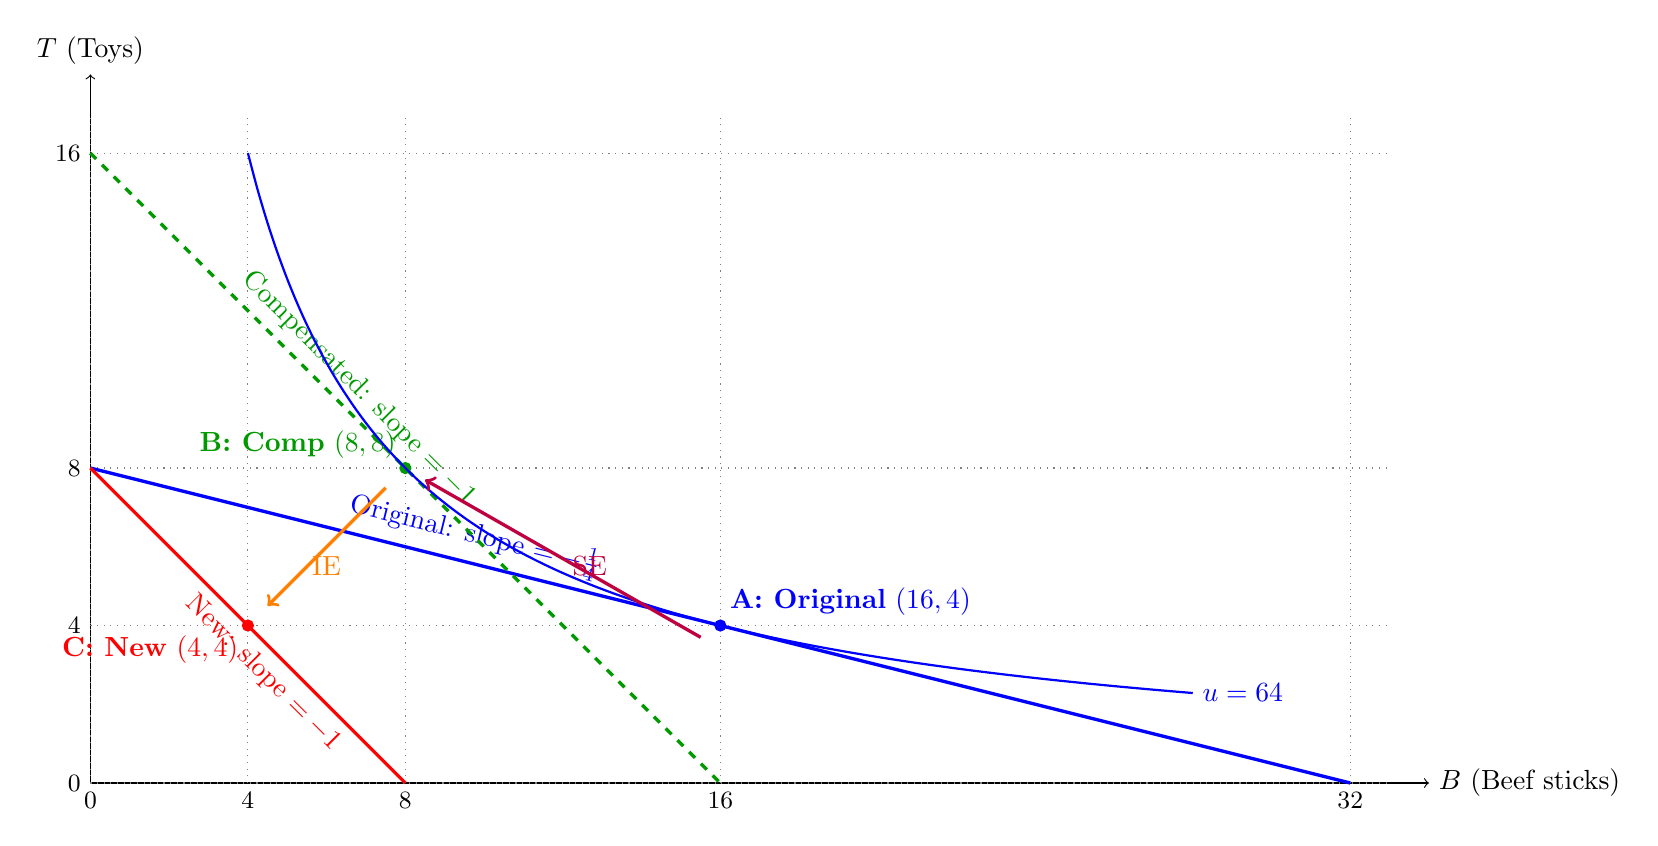
\begin{tikzpicture}[scale=0.5]
% Axes
\draw[->] (0,0) -- (34,0) node[right] {$B$ (Beef sticks)};
\draw[->] (0,0) -- (0,18) node[above] {$T$ (Toys)};

% Grid for reference
\foreach \x in {0,4,8,16,32} {
    \draw[dotted, gray] (\x, 0) -- (\x, 17);
    \node[below] at (\x, 0) {\small $\x$};
}
\foreach \y in {0,4,8,16} {
    \draw[dotted, gray] (0, \y) -- (33, \y);
    \node[left] at (0, \y) {\small $\y$};
}

% Original budget line: B + 4T = 32, so T = 8 - B/4
% T-int = 8, B-int = 32
\draw[very thick, blue] (0, 8) -- (32, 0) node[pos=0.3, above, sloped] {Original: slope $= -\frac{1}{4}$};

% New budget line: 4B + 4T = 32, so T = 8 - B
% T-int = 8, B-int = 8
\draw[very thick, red] (0, 8) -- (8, 0) node[pos=0.6, below, sloped] {New: slope $= -1$};

% Compensated: 4B + 4T = 64, so T = 16 - B
% T-int = 16, B-int = 16
\draw[very thick, green!60!black, dashed] (0, 16) -- (16, 0) node[pos=0.4, above, sloped] {Compensated: slope $= -1$};

% Points
\filldraw[blue] (16, 4) circle (4pt) node[above right] {\textbf{A: Original} $(16,4)$};
\filldraw[red] (4, 4) circle (4pt) node[below left] {\textbf{C: New} $(4,4)$};
\filldraw[green!60!black] (8, 8) circle (4pt) node[above left] {\textbf{B: Comp} $(8,8)$};

% Indifference curve u = 64
\draw[thick, blue, domain=4:28, smooth, samples=100] plot (\x, {64/\x});
\node[blue, right] at (28, 64/28) {$u=64$};

% Arrows showing effects
\draw[->, very thick, purple] (15.5, 3.7) -- (8.5, 7.7);
\node[purple, right] at (12, 5.5) {SE};

\draw[->, very thick, orange] (7.5, 7.5) -- (4.5, 4.5);
\node[orange, below] at (6, 6) {IE};

\end{tikzpicture}
\end{center}

\newpage

\section*{Why Each Line is Where It Is}

\subsection*{1. Why is the original line flatter?}

\textbf{Slope = $-\frac{p_B}{p_T} = -\frac{1}{4}$}

When beef costs \$1 and toys cost \$4, you only give up $\frac{1}{4}$ of a toy to get 1 beef stick. The line is relatively flat.

\subsection*{2. Why does the new line rotate inward?}

\textbf{Slope = $-\frac{p_B}{p_T} = -\frac{4}{4} = -1$}

When beef costs \$4 and toys cost \$4, you give up exactly 1 toy to get 1 beef stick. The line gets steeper.

\textbf{Why inward?} Because beef got more expensive, you can afford less beef. The B-intercept shrinks from 32 to 8.

\textbf{Why same T-intercept?} Toy price didn't change, so if you spend all money on toys, you can still buy 8 toys.

\subsection*{3. Why is the compensated line parallel to the new line?}

\textbf{Same slope = $-1$} because it uses the same new prices ($p_B = p_T = 4$).

\textbf{But shifted out} because we give Melsi \$64 instead of \$32, so she can afford more of everything.

\subsection*{4. Why does the compensated line pass through $(8,8)$?}

Because that's the cheapest bundle at new prices that achieves $u = 64$.

\section*{Summary Table}

\begin{center}
\begin{tabular}{|l|c|c|c|c|}
\hline
\textbf{Budget Line} & \textbf{Prices} & \textbf{Income} & \textbf{Slope} & \textbf{Optimal Point} \\
\hline
Original & $(1, 4)$ & \$32 & $-\frac{1}{4}$ & $(16, 4)$ \\
\hline
New & $(4, 4)$ & \$32 & $-1$ & $(4, 4)$ \\
\hline
Compensated & $(4, 4)$ & \$64 & $-1$ & $(8, 8)$ \\
\hline
\end{tabular}
\end{center}

\section*{The Key Insight}

\begin{center}
\colorbox{yellow!30}{
\begin{minipage}{0.9\textwidth}
\textbf{The compensated budget line is NOT real!}

It's a hypothetical line showing: ``What if we gave Melsi enough money to stay at $u=64$ after the price change?''

In reality, Melsi goes from the Original line to the New line. The Compensated line is just a tool to separate SE and IE.
\end{minipage}
}
\end{center}

\section*{Common Mistakes}

\begin{enumerate}
    \item \textbf{Thinking all three lines pass through the same point} - They don't! Each has a different optimal bundle.

    \item \textbf{Confusing which line uses which income} - Original and New use \$32; Compensated uses \$64.

    \item \textbf{Thinking the compensated line uses old prices} - No! It uses new prices with more income.

    \item \textbf{Not understanding why slopes change} - Slope $= -\frac{p_1}{p_2}$, so when relative prices change, slope changes.
\end{enumerate}

\end{document}
